\section{Backend}

\subsection{Overview}
The backend of FlowX uses a microservices architecture for scalability and modularity. It consists of:
\begin{itemize}
\item \textbf{API Microservice}: Handles authentication, workflow, and state management.
\item \textbf{Executor Microservice}: Executes LangChain logic.
\item \textbf{Infrastructure Service}: Manages deployment with Terraform and Kubernetes.
\end{itemize}

The following figure shows the API schema for the backend that allows Workflow creation:
\begin{figure}[H]
    \centering
    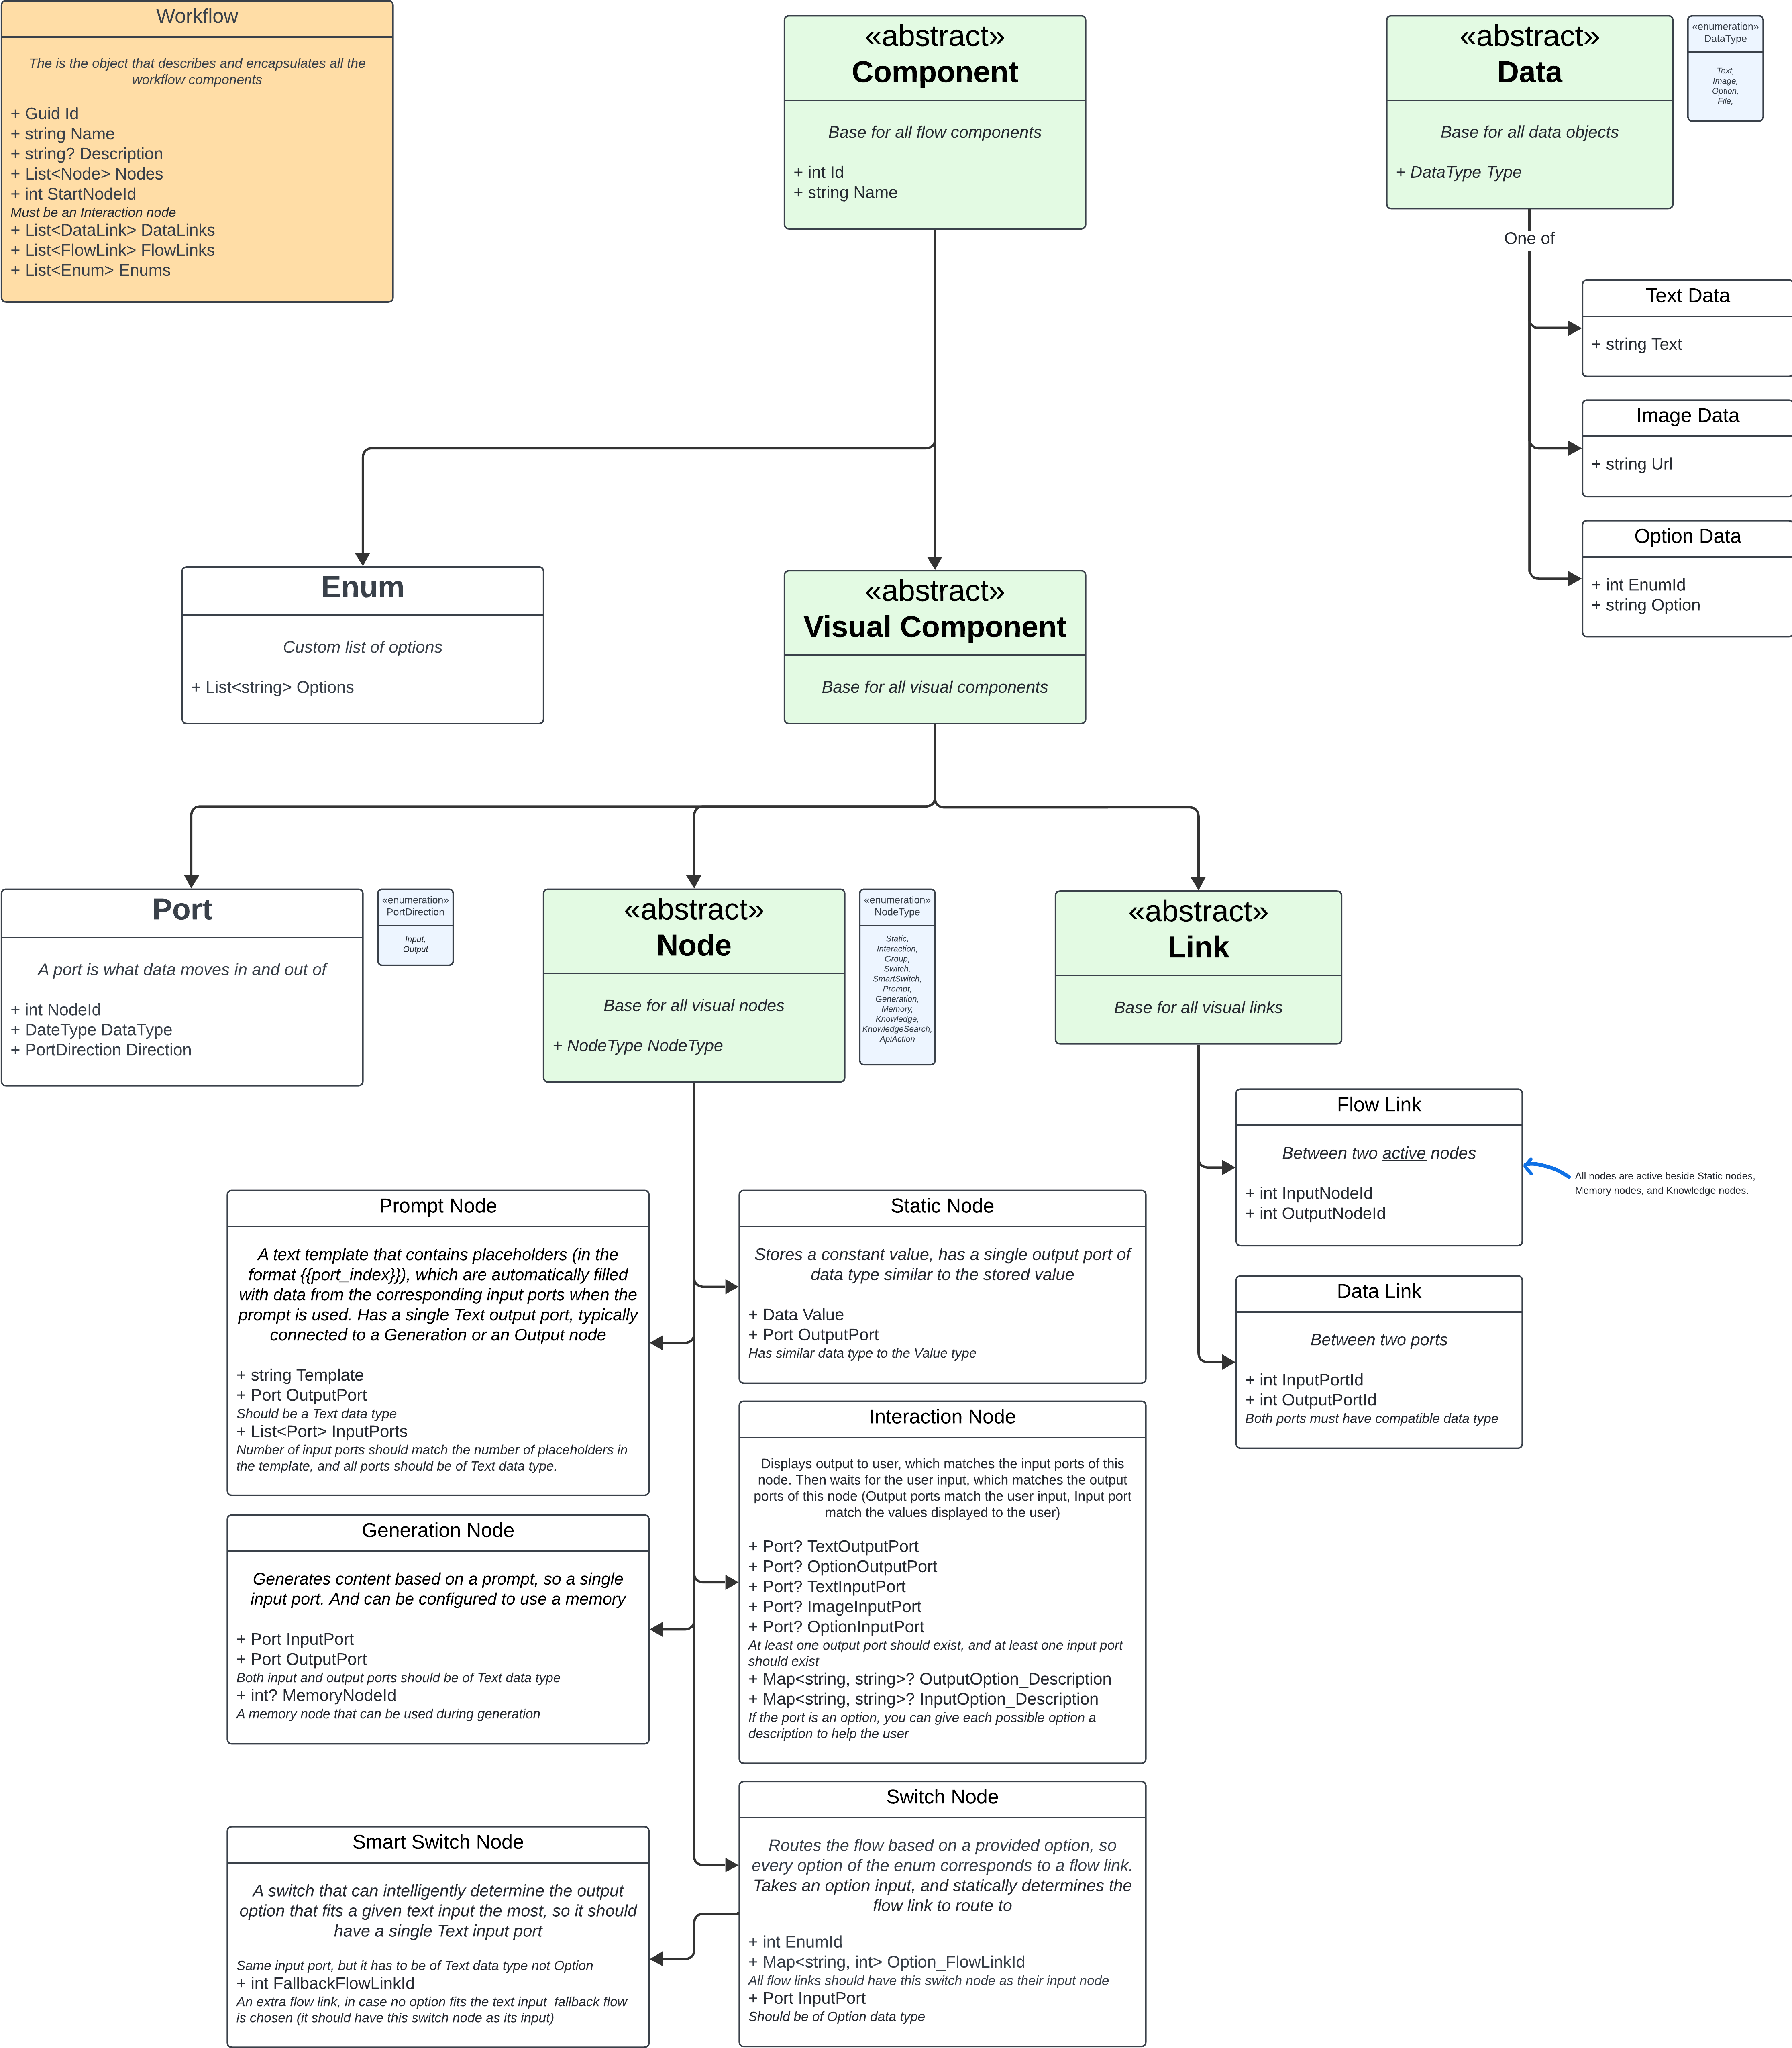
\includegraphics[width=0.95\textwidth]{assets/ChatbotBuilderApiSchema}
    \caption{API Schema for Chatbot Builder Workflows}
    \label{fig:api_schema}
\end{figure}

\subsection{API Microservice}
Built with \textbf{ASP.NET Core}, this service handles:
\begin{itemize}
\item \textbf{Authentication}: Uses JWT-based security.
\item \textbf{Workflow Management}: Supports CRUD operations.
\item \textbf{State Management}: Tracks chatbot workflow states.
\item \textbf{Executor Communication}: Delegates execution via gRPC.
\end{itemize}

\subsection{Domain Model}
The API service implements a rich domain model to support both user management and chatbot workflow functionality. Figure \ref{fig:system_uml} shows the core domain entities and their relationships.

\begin{figure}[H]
    \centering
    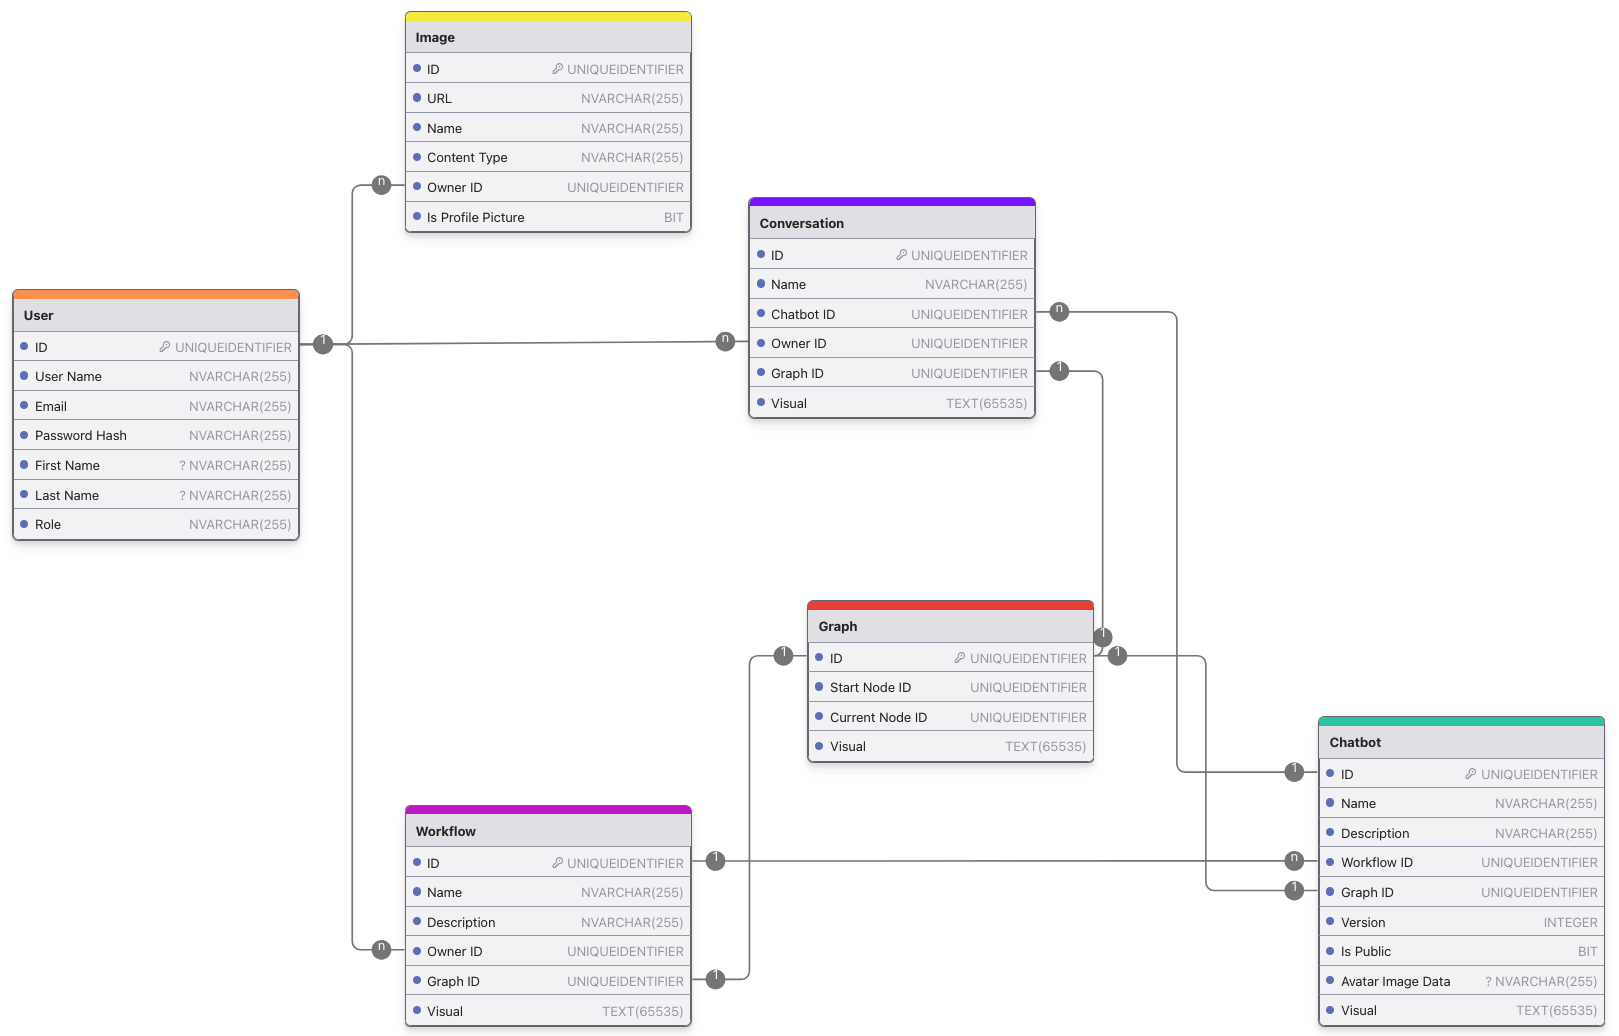
\includegraphics[width=0.95\textwidth]{assets/SystemUmlDiagram.png}
    \caption{Core Domain Model Class Diagram}
    \label{fig:system_uml}
\end{figure}

The domain model is centered around these key entities:
\begin{itemize}
    \item \textbf{User}: Manages authentication and profile data, including role-based access control
    \item \textbf{Chatbot}: Encapsulates chatbot configuration and references to its workflow implementation
    \item \textbf{Workflow}: Contains the complete chatbot logic as a graph structure
    \item \textbf{Graph}: Maintains the topology of nodes and connections that define the chatbot's behavior
    \item \textbf{Conversation}: Handles state management for ongoing user interactions
\end{itemize}

\subsection{Graph Implementation}
The workflow execution engine is built on a sophisticated graph structure (Figure \ref{fig:graph_uml}) that enables both static flows and dynamic LLM-powered interactions.

\begin{figure}[H]
    \centering
    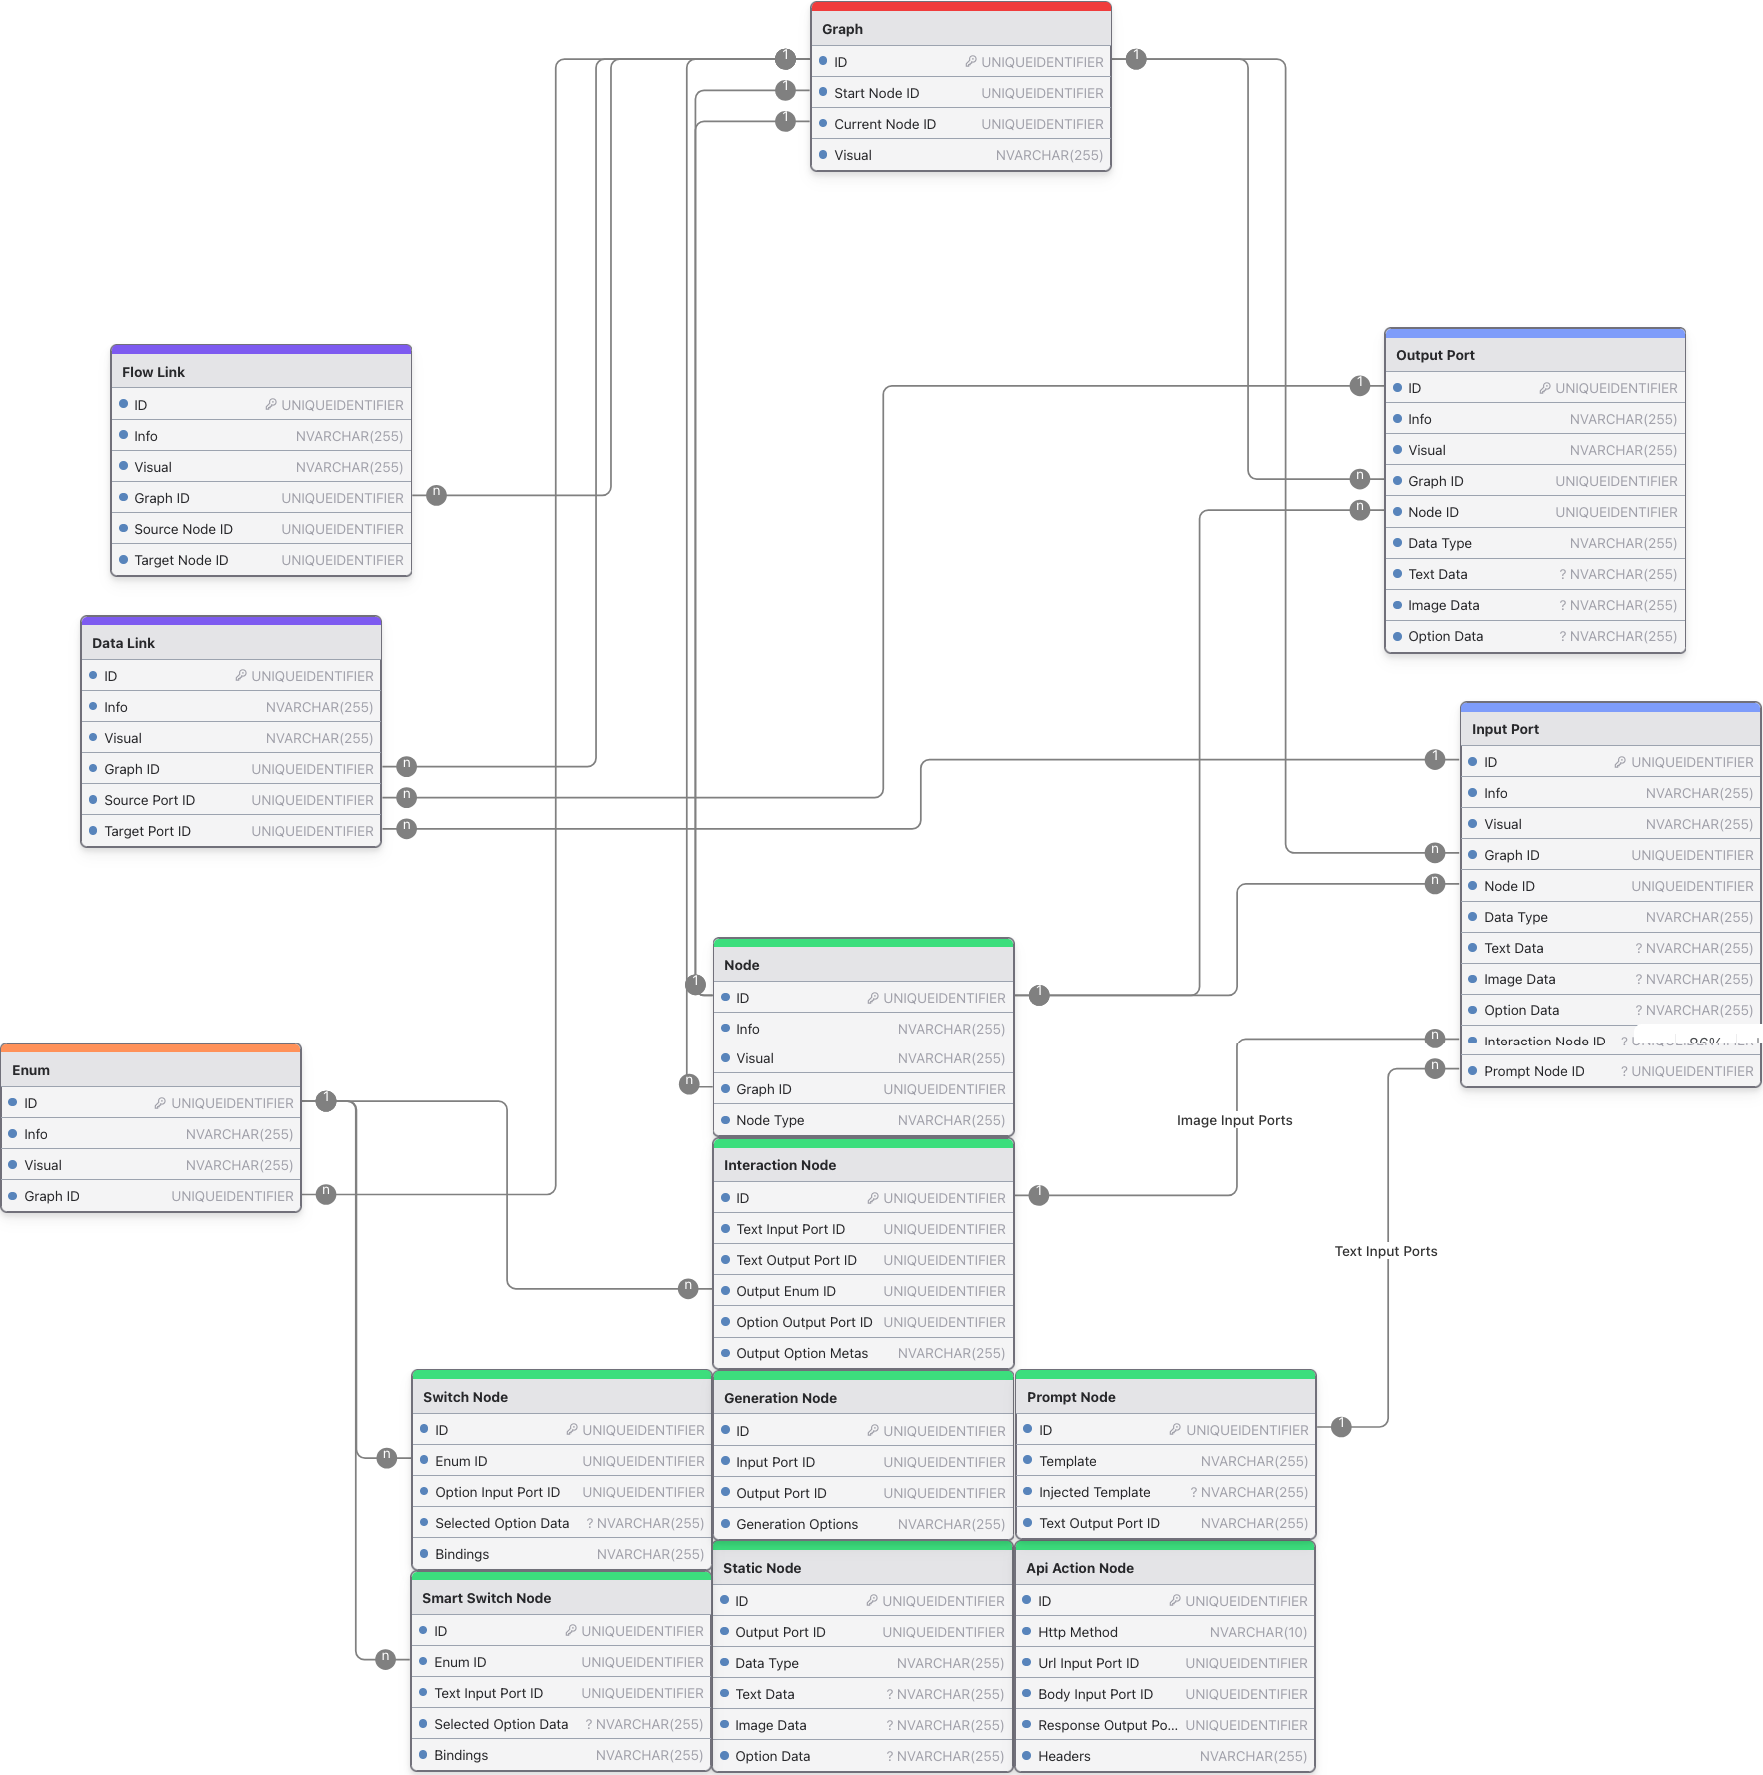
\includegraphics[width=0.95\textwidth]{assets/GraphUmlDiagram.png}
    \caption{Graph Implementation Class Diagram}
    \label{fig:graph_uml}
\end{figure}

The graph implementation includes:
\begin{itemize}
    \item \textbf{Node}: Abstract base class defining common node behavior
    \item \textbf{Input/Output Ports}: Strongly-typed connection points enabling type-safe data flow
    \item \textbf{Flow/Data Links}: Distinct connection types for control flow vs data transfer
    \item \textbf{Specialized Nodes}:
    \begin{itemize}
        \item \textbf{Interaction Node}: Manages user input/output with templating support
        \item \textbf{Generation Node}: Interfaces with the Executor service for LLM operations
        \item \textbf{Switch Node}: Implements both static and LLM-powered conditional branching
        \item \textbf{Static Node}: Provides deterministic responses
        \item \textbf{API Action Node}: Enables integration with external services
    \end{itemize}
\end{itemize}

\subsection{Executor Microservice}
Developed in \textbf{Python} with \textbf{LangChain}, responsible for:
\begin{itemize}
\item \textbf{Chatbot Logic Execution}.
\item \textbf{gRPC Communication} with the API service.
\item \textbf{Handling Smart Switch Nodes} using LLM outputs.
\end{itemize}

\subsection{Infrastructure and Deployment}
Managed using \textbf{Terraform} and \textbf{Kubernetes}, ensuring:
\begin{itemize}
\item \textbf{Scalable Deployment}: Kubernetes handles scaling and failover.
\item \textbf{Infrastructure as Code (IaC)}: Terraform automates provisioning.
\item \textbf{Service Communication}: Uses gRPC and RESTful APIs.
\end{itemize}